\documentclass[letterpaper]{article}
% generated by Docutils <http://docutils.sourceforge.net/>
\usepackage{fixltx2e} % LaTeX patches, \textsubscript
\usepackage{cmap} % fix search and cut-and-paste in Acrobat
\usepackage{ifthen}
\usepackage[T1]{fontenc}
\usepackage[utf8]{inputenc}
\usepackage{amsmath}
\usepackage{float} % float configuration
\floatplacement{figure}{H} % place figures here definitely
\usepackage{graphicx}
\setcounter{secnumdepth}{0}
\usepackage{longtable,ltcaption,array}
\setlength{\extrarowheight}{2pt}
\newlength{\DUtablewidth} % internal use in tables
\usepackage{tabularx}

%%% Custom LaTeX preamble
% PDF Standard Fonts
\usepackage{mathptmx} % Times
\usepackage[scaled=.90]{helvet}
\usepackage{courier}

%%% User specified packages and stylesheets
\usepackage{fullpage}
\usepackage{microtype}
\usepackage[htt]{hyphenat}

%%% Fallback definitions for Docutils-specific commands

% providelength (provide a length variable and set default, if it is new)
\providecommand*{\DUprovidelength}[2]{
  \ifthenelse{\isundefined{#1}}{\newlength{#1}\setlength{#1}{#2}}{}
}

% docinfo (width of docinfo table)
\DUprovidelength{\DUdocinfowidth}{0.9\textwidth}

% hyperlinks:
\ifthenelse{\isundefined{\hypersetup}}{
  \usepackage[colorlinks=true,linkcolor=blue,urlcolor=blue]{hyperref}
  \urlstyle{same} % normal text font (alternatives: tt, rm, sf)
}{}
\hypersetup{
  pdftitle={CS 452 P2},
}

%%% Title Data
\title{\phantomsection%
  CS 452 P2%
  \label{cs-452-p2}}
\author{}
\date{}

%%% Body
\begin{document}
\maketitle

% Docinfo
\begin{center}
\begin{tabularx}{\DUdocinfowidth}{lX}
\textbf{Names}: &
Robert Elder, Christopher Foo
\\
\textbf{ID \#}: &
20335246, 20309244
\\
\textbf{Userids}: &
relder, chfoo
\\
\textbf{Date due}: &
July 23, 2013
\\
\end{tabularx}
\end{center}


\section{Running%
  \label{running}%
}

The executable is located at \texttt{/u/cs452/tftp/ARM/relder-chfoo/p2-submit/kern.elf}.

The entry point is located at \texttt{0x00045000} or \texttt{\%\{FREEMEMLO\}} It \emph{must} be executed with caching enabled. (Caches not enabled by the program itself due to time contraints):
%
\begin{quote}{\ttfamily \raggedright \noindent
load~-b~\%\{FREEMEMLO\}~-h~10.15.167.4~ARM/relder-chfoo/p2-submit/kern.elf\\
go~-c
}
\end{quote}


\subsection{Commands%
  \label{commands}%
}
%
\begin{description}
\item[{tr TRAIN SPEED}] \leavevmode 
Set the train speed.

\item[{rv TRAIN}] \leavevmode 
Slows, stops, and reverses train. The final speed is hard coded to 5.

\item[{sw SWITCH DIRECTION}] \leavevmode 
Changes the turnout direction. DIRECTION is either S or C.

\item[{q}] \leavevmode 
Quits the program.

\item[{map NAME}] \leavevmode 
Sets the current track. NAME should be A or B.

\end{description}

Figure 2 and Figure 3 show different map configurations.
\begin{figure}
\noindent\makebox[\textwidth][c]{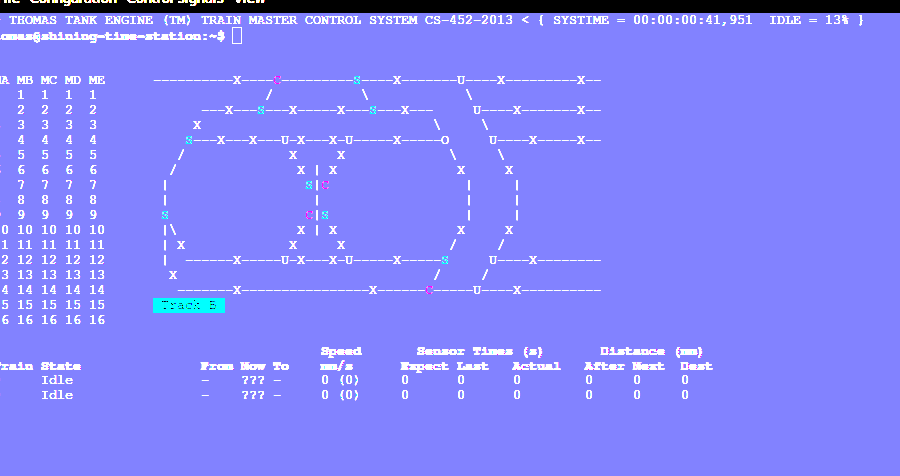
\includegraphics[width=\textwidth]{figure2.png}}
\caption{Figure 2}
\end{figure}
%
\begin{description}
\item[{go TRAIN}] \leavevmode 
Begins the train route finding process. The train should start up, find position, and go to a random destination.

\item[{gf TRAIN}] \leavevmode 
Like \texttt{go}, however, this make the train go forever by running \texttt{go} in an continuous loop.

\item[{num TRAINS}] \leavevmode 
Set the number of trains to be used.

\item[{paint}] \leavevmode 
Causes the interface to redraw itself.

\item[{rt}] \leavevmode 
Resets the train system by stopping the trains, clearing reservations, and clearing train engine states.

\item[{rps}] \leavevmode 
Runs Rock Paper Scissors program.

\end{description}

Pressing 'CTRL+Z' will cause the program to dump out a list of tasks information and statistics.   This is considered a debug operation, and as such it can cause future instability in the program.

Pressing CTRL+C will cause the program to exit immediately without shutting down the tasks.


\subsubsection{Getting Started Quickly%
  \label{getting-started-quickly}%
}

To start up two trains
\newcounter{listcnt0}
\begin{list}{\arabic{listcnt0}.}
{
\usecounter{listcnt0}
\setlength{\rightmargin}{\leftmargin}
}

\item Select the appropriate map using the \texttt{map} command.

\item Set the number of trains to be used using \texttt{num} command.

\item Enter the first train using \texttt{go TRAINNUM1 0}

\item Enter the second train using \texttt{go TRAINNUM2 1}

\item If things go wrong, use the \texttt{rt} command
\end{list}


\section{Description%
  \label{description}%
}


\subsection{Kernel%
  \label{kernel}%
}
%
\begin{itemize}

\item No kernel changes since last deliverable.

\end{itemize}
\begin{figure}
\noindent\makebox[\textwidth][c]{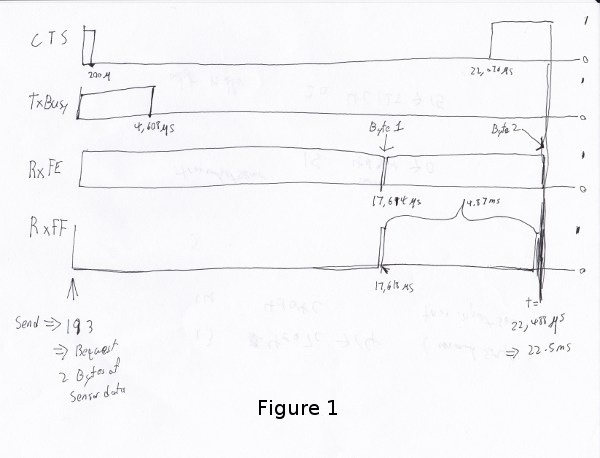
\includegraphics[width=\textwidth]{figure1.jpg}}
\end{figure}


\subsubsection{System Calls%
  \label{system-calls}%
}
%
\begin{itemize}

\item System calls support up to 5 arguments.

\item No changes since last deliverable.

\end{itemize}
%
\begin{description}
\item[{\texttt{Create}}] \leavevmode 
Returns the new task id, \texttt{ERR\_K\_INVALID\_PRIORITY -1}, or \texttt{ERR\_K\_OUT\_OF\_TD -2}

\item[{\texttt{MyTid}}] \leavevmode 
Returns the current task id

\item[{\texttt{MyParentTid}}] \leavevmode 
Returns the parent task id. The parent task id is always returned regardless of the parent's state.

\item[{\texttt{Pass}}] \leavevmode 
(Rescheduling happens as normal in the background.)

\item[{\texttt{Exit}}] \leavevmode 
Task is marked as \texttt{ZOMBIE} (and rescheduling happens as normal in the background).

\item[{\texttt{Send}}] \leavevmode 
Sends a message to the given task ID. \texttt{-3} code is not implemented.

\item[{\texttt{Receive}}] \leavevmode 
Blocks until a message is received. Returns the size of the message which will be typically \texttt{MESSAGE\_SIZE 16}

\item[{\texttt{Reply}}] \leavevmode 
Replies a message to the task. On errors \texttt{-3} \texttt{-4}, an assert will fire before returning to aid in debugging.

\item[{\texttt{RegisterAs}}] \leavevmode 
Prepares a \texttt{NameServerMessage} structure with a message type of \texttt{REGISTER\_AS} and sends the message to the Name Server. \texttt{0} is always returned because the Task ID is hard-coded and the call should never send to the wrong task.

\item[{\texttt{WhoIs}}] \leavevmode 
Prepares a \texttt{WHO\_IS} message type and sends it to the Name Server. As noted in \texttt{RegisterAs}, we either return a Task ID or 0 if the task has not been created. However, the task ID returned may be in a zombie state.

\item[{\texttt{AwaitEvent}}] \leavevmode 
Marks the task as \texttt{EVENT\_BLOCKED}. The task will be unblocked by the Scheduler. This call always returns 0 and the user task will be responsible for obtaining the data themselves. \texttt{AwaitEvent} supports only 1 task per event type.

\item[{\texttt{Time}}] \leavevmode 
Wraps a \texttt{Send} to the Clock Server. It first queries the Name Server for the Clock Server and then sends a \texttt{TIME\_REQUEST} message. It expects back a \texttt{TIME\_REPLY} message and returns the time.

\item[{\texttt{Delay}}] \leavevmode 
Similar to \texttt{Time}, it sends a \texttt{DELAY\_REQUEST} message and expects back a \texttt{DELAY\_REPLY} message.

\item[{\texttt{DelayUntil}}] \leavevmode 
Similar to \texttt{Time}, it sends a \texttt{DELAY\_UNTIL\_REQUEST} message and expects back a \texttt{DELAY\_REPLY} message.

\item[{\texttt{TimeSeconds}, \texttt{DelaySeconds}, \texttt{DelayUntilSeconds}}] \leavevmode 
Same as above but in seconds. It simply converts the ticks into seconds before calling the system calls. These calls are simply for convenience.

\item[{\texttt{Getc}}] \leavevmode 
Sends a message to either Keyboard Input Server or Train Input Server. It will block until the servers have a character to return.

\item[{\texttt{Putc}}] \leavevmode 
Sends a message to either Screen Output Server or Train Output Server. The servers will place the character into the server's Char Buffer.

\item[{\texttt{PutString}}] \leavevmode 
Formats the string and calls \texttt{Putc} for every character.

\item[{\texttt{PutcAtomic}}] \leavevmode 
Like \texttt{Putc}, but accepts multiple characters and guarantees the characters are placed into the queue sequentially. This call is useful to ensure that two byte commands are not separated by a single byte command.

\item[{\texttt{SendTrainCommand}}] \leavevmode 
Sends a message type \texttt{TRAIN\_COMMAND} to the Train Command Server. The call is for convenience.

\item[{\texttt{PrintMessage}}] \leavevmode 
Similar to \texttt{PrintMessage}, but this sends the string to the UI Print Server to be displayed on the lower half of the screen using a \texttt{UI\_PRINT\_MESSAGE} message type

\end{description}


\subsubsection{Watchdog%
  \label{watchdog}%
}

The watchdog has been changed to report starvation after 500,000 schedules to be more strict in detecting this problem.


\subsubsection{Scheduler%
  \label{scheduler}%
}

The scheduler now calculates the system load by counting the number of low priority schedules per 1,000,000 schedules. This may not reflect the true load as the Idle Task may take a long time slice before rescheduling. In the future deliverable, we may implement counting the time each task is scheduled.


\subsubsection{Priorities%
  \label{priorities}%
}

For this deliverable, we have thought carefully about the priorities of each task.

\setlength{\DUtablewidth}{\linewidth}
\begin{longtable*}[c]{|p{0.296\DUtablewidth}|p{0.133\DUtablewidth}|}
\hline
\textbf{%
Task
} & \textbf{%
Priority
} \\
\hline
\endfirsthead
\hline
\textbf{%
Task
} & \textbf{%
Priority
} \\
\hline
\endhead
\multicolumn{2}{c}{\hfill ... continued on next page} \\
\endfoot
\endlastfoot

Clock Notifier
 & 
0
 \\
\hline

Clock Server
 & 
0
 \\
\hline

First Task
 & 
0
 \\
\hline

Name Server
 & 
1
 \\
\hline

Administrator
 & 
2
 \\
\hline

UART Bootstrap
 & 
3
 \\
\hline

Train IO Notifier
 & 
4
 \\
\hline

Train Input Notifier
 & 
4
 \\
\hline

Train Output Notifier
 & 
4
 \\
\hline

Keyboard Input Notifier
 & 
4
 \\
\hline

Screen Output Notifier
 & 
4
 \\
\hline

Train Input Server
 & 
5
 \\
\hline

Train Output Server
 & 
5
 \\
\hline

Screen Output Server
 & 
6
 \\
\hline

Keyboard Input Server
 & 
6
 \\
\hline

Train Server
 & 
7
 \\
\hline

UI Print Task
 & 
7
 \\
\hline

Train Command Server
 & 
8
 \\
\hline

Train Switch Master
 & 
8
 \\
\hline

UI Server
 & 
8
 \\
\hline

Train Sensor Reader
 & 
9
 \\
\hline

Train Engine
 & 
9
 \\
\hline

Train Server Timer
 & 
10
 \\
\hline

UI Keyboard Input
 & 
12
 \\
\hline

UI Timer
 & 
13
 \\
\hline

RPS Test Start
 & 
15
 \\
\hline

RPS Server
 & 
16
 \\
\hline

RPS Client
 & 
31
 \\
\hline

Idle Task
 & 
31
 \\
\hline
\end{longtable*}

For more info, see Performance.


\subsection{Assert%
  \label{assert}%
}

The assert statement, as usual, is enhanced to show Thomas The Tank Engine. Please do not be alarmed when you see it.

When an assertion failure occurs, the Stop command will now be sent to avoid train collisions.


\subsection{Serial IO%
  \label{serial-io}%
}

File: \texttt{uart.c}
%
\begin{itemize}

\item FIFOs are now used for the terminal input/output.

\end{itemize}


\subsection{Train Navigation%
  \label{train-navigation}%
}

File: \texttt{route.c}, \texttt{tracks/track\_data.c}, \texttt{train\_logic.c}, \texttt{train\_data\_structures.h}

Train navigation is currently accomplished using naive graph search algorithms, as well as a server called the SwitchMaster that is responsible for updating the positions of switches.

We have broken down the problem of navigation to anywhere on the map into two basic problems: The first is navigation to a point while considering the map as a directed graph.  In this situation we only consider moving in the forward direction.  In this context, it is not possible to navigate to anywhere on the map from all nodes because the graph is considered to be a directed one.  In the second case, we consider the map as an undirected graph, where any shortest path can be found by finding the shortest route in the undirected graph.  We can then express the problem of navigation between two points in the undirected graph as multiple navigations in a directed graph, while adding direction reversals in the middle.

To find a destination, a simple depth first recursive algorithm is used to build up a Route Info array. The Route Info array contains information about each track node and the switches it needs to switch. The algorithm avoids blacklisted switches.


\subsection{Undirected Graph Model%
  \label{undirected-graph-model}%
}

In order to accurately model the train and its motion around the track, as well as predicted future positions on the track, we required another representation of the track to complemented the directed model that was provided.  It is for this reason that we have created a undirected graph model of the track based on the directed graph model.  This model also includes the trains as nodes, which enables us to apply standard graph-based algorithms to any nodes on the track graph, including the trains themselves.  This has significant advantages for tasks such as sensor attribution, collision detection, and route planning.  The advantage of including the trains as nodes in this model means that in this representation, we do not need sensor data to make decisions about what actions to take, and can rely on the current state of the model that has been predicted based on last sensor observations.  The undirected graph model allows us to consider route planning, independent of the number of reversals that are required on the route.  The other advantage is that trains are included as nodes so that the shortest distance between two trains can be calculated down to the micrometer at any point in time, as long as their approximate speed is known.

Sensor triggering can be used to infer observed train speeds, which can be used to simulate the motion of the train in a near continuous time manner.


\subsection{Undirected Graph Data Structure%
  \label{undirected-graph-data-structure}%
}

The undirected graph model is built from the directed track node data.  Pointers are added to the directed nodes that point to the corresponding undirected graph nodes, and vice versa.  The undirected graph model is implemented as an adjacency list.  Since every node in this graph can have a maximum of 3 adjacent nodes, this significantly shortens the run time and memory requirements of many graph processing algorithms.


\subsubsection{Dijkstra's%
  \label{dijkstra-s}%
}

Dijkstra's algorithm has been implemented for the undirected graph nodes.  The implementation of this algorithm is the standard one, with a run-time of $O(|E| + |V|)$.  Testing has been done with a simulated track where multiple trains are sent on a random-walk around the track millions of times, calculating the shortest distance at each step.  Valgrind was also used to preclude the possibility of programming errors.


\subsubsection{Routing and Navigation%
  \label{routing-and-navigation}%
}

Currently, we use a simple recursive graph search algorithm for calculating paths.  This will soon be replaced by the much more accurate Dijkstra's algorithm once the undirected graph model is incorporated into the routing.  Once we have determined a series of nodes that we need to navigate through, we determine the set of switches that need to be changed from their current state, up until we possibly end up changing that same switch again (for re-entrant paths that only involve moving forward).  The switches are queued in the order in which they need to be switched so that the closest switch will be the first one to change.  If the train triggers a sensor that is not on the path it was expected to take, a warning is printed for debugging purposes.


\subsubsection{Stopping%
  \label{stopping}%
}

For stopping we use a roughly approximated table for each train that will tell us how many millimeters before a sensor we need to issue a command to slow down.  This table was derived from empirical measurements and still needs a bit of calibration.  This is especially true on a specific train level, since different trains require different stopping distances.

A list of speeds for each node during stopping has also been determined empirically. Nodes that are near switches have a lower speed to avoid stopping on top of a switch. We risk the trains getting stuck on curves because it is preferred that trains become stuck rather than derailed by an activating switch.


\subsubsection{Velocity%
  \label{velocity}%
}

Our trains move at a speed of 45 cm/s and we maintain this speed using a feedback control mechanism. The observed train speed is calculated by dividing the known track length between two sensors, and dividing this by the observed time taken to travel between them.  The trains use a floating point speed setting to avoid sending too many train speed commands and to dampen noise. The floating point speed setting is casted to an int and the command is issued if needed. The algorithm slowly increases the train speed when it arrives at a sensor too slowly, and decreases the speed quickly when it arrives too fast.


\subsubsection{Sensor Malfunctions%
  \label{sensor-malfunctions}%
}

Sensor malfunctions are accounted for by maintaining a list of sensors that are known to malfunction on each track.  We use a blacklist of sensors to remember which sensors should not be navigated to, and which should be ignored when determining the train position.


\subsubsection{Reservations%
  \label{reservations}%
}

The provided track nodes have been modified with an extra field called \texttt{reserved}. It holds the train number of the reservation. Once the destination and route is calculated, all the nodes in the route are reserved. Once the train reaches its destination, the nodes are released from reservation.  The concept of switch reservations is taken care of, because while a train has reserved a switch, no other can attempt to queue a switch change.


\subsubsection{Train Switch Master%
  \label{train-switch-master}%
}

The Switch Master is responsible for picking up switch commands from the Train Server and calling Train Command Server. This task is a worker that removes the burden of waiting for train commands to complete.


\subsubsection{Train Engine Client%
  \label{train-engine-client}%
}

The Engine Client is responsible for picking up train speed commands from the Train Server and calling the Train Command Server. Like the Switch Master, the task is a worker hired by the Train Server.


\subsubsection{Train Engine States%
  \label{train-engine-states}%
}

\setlength{\DUtablewidth}{\linewidth}
\begin{longtable*}[c]{|p{0.321\DUtablewidth}|p{0.619\DUtablewidth}|}
\hline
\textbf{%
Name
} & \textbf{%
Description
} \\
\hline
\endfirsthead
\hline
\textbf{%
Name
} & \textbf{%
Description
} \\
\hline
\endhead
\multicolumn{2}{c}{\hfill ... continued on next page} \\
\endfoot
\endlastfoot

IDLE
 & 
The engine is stopped and waiting.
 \\
\hline

FINDING\_POSITION
 & 
The engine is moving slowly and waiting for a sensor
 \\
\hline

RESYNC\_POSITION
 & 
The engine has drifted from its calculated position and
is attempting to find its location
 \\
\hline

FOUND\_STARTING\_POSITION
 & 
The engine has found its location
 \\
\hline

WAIT\_FOR\_DESTINATION
 & 
The engine is waiting for a destination to be calculated
 \\
\hline

GOT\_DESTINATION
 & 
The engine has calculated its destination
 \\
\hline

WAIT\_FOR\_ALL\_READY
 & 
The engine is waiting for other engines to be found and ready
 \\
\hline

RUNNING
 & 
The engine is running at high speeds to the destination
 \\
\hline

AT\_DESTINATION
 & 
The engine is at the destination and stopped.
 \\
\hline

NEAR\_DESTINATION
 & 
The engine has slowed down and is waiting for a
sensor report.
 \\
\hline

REVERSE\_AND\_TRY\_AGAIN
 & 
The engine is in a direction that provides no
destination and is reversing to find a new
sensor.
 \\
\hline

WAIT\_FOR\_RESERVATION
 & 
The engine has stopped and is waiting for the track to become
unreserved
 \\
\hline

WRONG\_LOCATION
 & 
The engine has entered an unauthorized section of the track
 \\
\hline
\end{longtable*}


\subsubsection{GO%
  \label{go}%
}

The go command operates as following:
\setcounter{listcnt0}{0}
\begin{list}{\arabic{listcnt0}.}
{
\usecounter{listcnt0}
\setlength{\rightmargin}{\leftmargin}
}

\item Set the train speed to 5.

\item If a sensor is hit, the location of the train has been found.

\item Reserve the current location in the reservation system.

\item If there are other trains that need to find their location, wait for them.

\item Pick a random destination.

\item Calculate a route to the destination.

\item If there is no possible route to destination, reverse the direction and go to step 5.

\item Activate the switches that do not overlap other routes or require switching multiple times.

\item Speed up the train to 14.

\item Read sensors and compute the speed, location, and distance to update the state of the train engine.

\item Using the sensor data and  feedback control system, adjust the speed to achieve a speed of 45 cm/s.

\item If the next node is a switch that needs to be activated, switch it.

\item If the distance to destination is within the stopping distance, slow the train down.

\item Wait for a sensor and stop.
\end{list}

For an iterative version of the go command, see GF command which will iteratively use the go command after a train reaches its destination.


\subsubsection{GF%
  \label{gf}%
}

The gf command operates as following:
\setcounter{listcnt0}{0}
\begin{list}{\arabic{listcnt0}.}
{
\usecounter{listcnt0}
\setlength{\rightmargin}{\leftmargin}
}

\item Do steps 1-14 of the go command

\item Wait for 4 seconds

\item Goto step 1
\end{list}


\subsection{UI Servers%
  \label{ui-servers}%
}

Files used by UI servers: \texttt{ui.c}, \texttt{ansi.c}, \texttt{maps/map\_gen.py}, \texttt{maps/map\_a.txt}, \texttt{maps/map\_b.txt}


\subsubsection{UI Server%
  \label{ui-server}%
}
%
\begin{itemize}

\item CR LF is handled correctly now.

\item Minor bug: certain inputs will cause assertion failures.

\end{itemize}

The UI Server is responsible for drawing the textual user interface. It draws a header, the time since start up, a system load indicator expressed in percentage, the command prompt, table of sensors readings, an ASCII diagram of the track layout, a table of train status, and a scrolled area of train information.

The command prompt supports up to 80 characters. Once this limit is reached, no input will be accepted and displayed. It supports backspace. Pressing the Enter key will execute the command and a response will be displayed under the command prompt. If an error occurs, it will be shown in yellow.

When a sensor is triggered, the UI Server will display an bold number on the table. Sensor data for the UI is cached by the Train Server so displayed sensor readings may not reflect actual state. Sensor states in the Train Server, however, reflect actual states.

The ASCII map shows sensors as X and bold X. Switches are shown as U, C, or S which represent Unknown, Curved, or Straight. The ASCII map code was generated through a script from a text file.

A green highlight shows the destination of the first train. A yellow highlight shows the destination for other trains.

A black highlight shows the reservation of the first train. A red highlight shows the reservation for other trains.

Some of the hilights of the UI are found in figure 4.
\begin{figure}
\noindent\makebox[\textwidth][c]{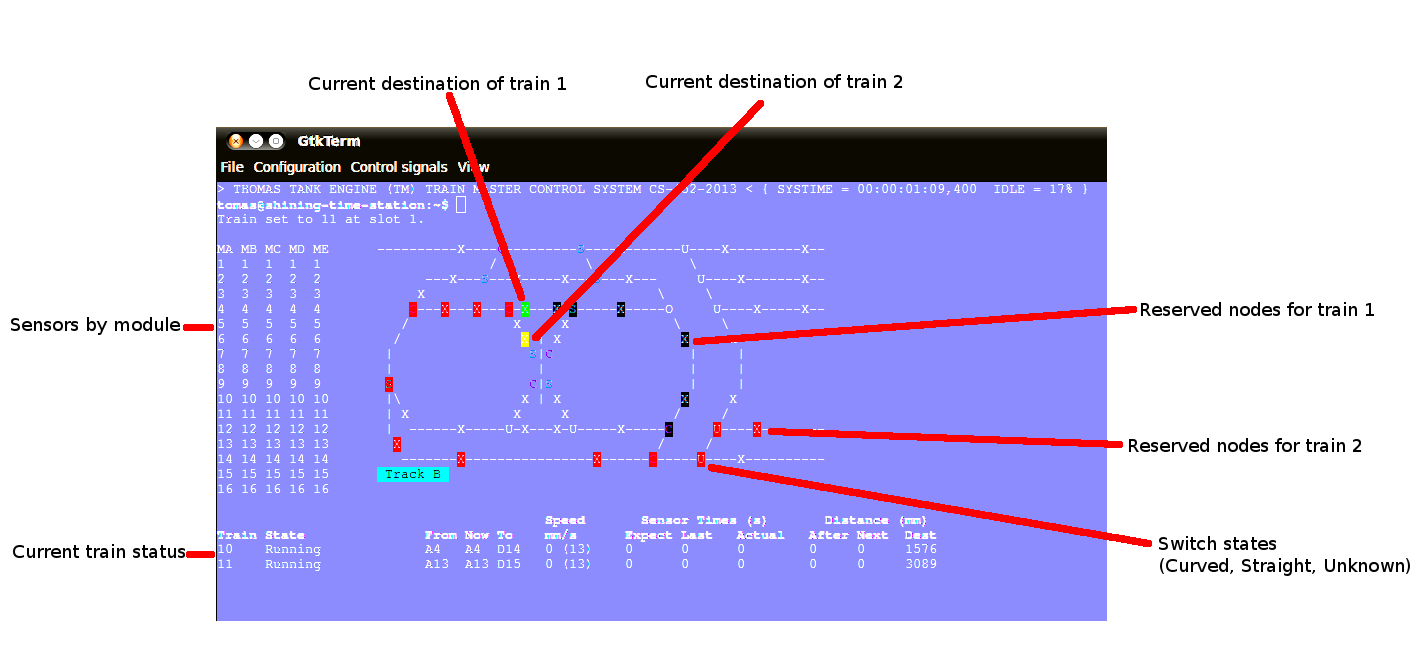
\includegraphics[width=\textwidth]{figure4.png}}
\caption{Figure 4}
\end{figure}


\subsubsection{UI Timer%
  \label{ui-timer}%
}

The UI Timer is responsible for sending a message to the UI Server. The timer tells the UI to update the clock and system load on the screen.


\subsubsection{UI Keyboard Input Task%
  \label{ui-keyboard-input-task}%
}

The UI Keyboard Input task is responsible for calling \texttt{Getc} and sending the character to the UI Server.


\subsubsection{UI Print Message Task%
  \label{ui-print-message-task}%
}

This task is responsible for printing messages into the scrolled area. It uses the ANSI feature to set scrolling areas. It is separate from the UI Server as messages may be from higher priority tasks like the Train Server. It is called via the \texttt{PrintMessage} call.  This method was implemented as a non busy-waiting alternative for debug messages.


\subsubsection{Rock Paper Scissors%
  \label{rock-paper-scissors}%
}

Rock Paper Scissors is now back and can be run using the \texttt{rps} command.  Since it still functions from our earlier deliverable, we have decided to use it for stress testing.  It currently runs with 42 clients players.  It will display the results of each round in the scrolling area of the UI. The \texttt{rps} command should only be run once, however, the RPS games will last 12345689 rounds so there is no need to rerun the \texttt{rps} command the second time.


\subsection{Performance%
  \label{performance}%
}

In this deliverable we have several features that significantly improve the performance of our kernel:
\setcounter{listcnt0}{0}
\begin{list}{\arabic{listcnt0})}
{
\usecounter{listcnt0}
\setlength{\rightmargin}{\leftmargin}
}

\item The priorities were adjusted to achieve the following
%
\begin{itemize}

\item Notifiers have high priority

\item The UI keyboard input no longer drops characters while the UI is redrawing.

\item The Switch Master and Train Speed Client are at higher priorities than the Sensor Reader. This setup is necessary to avoid the trains getting caught on the switches.

\end{itemize}

\item FIFOs for the terminal were enabled. Without FIFOs, the UI task may be interrupted during sending ANSI sequences and leaving incomplete sequences on the screen. With FIFOs, the screen updates correctly without flickering.
\end{list}


\section{Source Code%
  \label{source-code}%
}

The source code is located at \texttt{/u4/chfoo/cs452/group/p2-submit/io/project2/}. It can be compiled by running \texttt{make}.

Source code MD5 hashes:
%
\begin{quote}{\ttfamily \raggedright \noindent
chfoo@nettop36:\textasciitilde{}/cs452/group/p2-submit/io/project2\$~md5sum~*/*/*~*/*.*~~*.*\\
bd0a0df5b9fbc588bdc203efe3c6570d~~tracks/tests/Makefile\\
fac587c527e77d0b2b243879ce9cc9a3~~tracks/tests/tests.c\\
50ef0e1e3c71ab1e795fc3d39f75ef9d~~include/bwio.h\\
9af226f127c1fd759530cd45236c37b8~~include/ts7200.h\\
94944e9febc4db1bb344fff990ed7e9e~~maps/map.h\\
3dfa3ed141445a72c20840b384c1ebb9~~maps/map\_a.c\\
c6adb76c95a6ae7986d03cd416d5837e~~maps/map\_a.h\\
703f1eeadf245074517591baa0844a37~~maps/map\_a.txt\\
c415ff53472ff6ffcd28afcab0038e4c~~maps/map\_b.c\\
eba8710b29615da70e7165571efd99d8~~maps/map\_b.h\\
093b6fff35ab1def4b776eb25a623c01~~maps/map\_b.txt\\
ead84e8315fd7e45f0e8e631197b9150~~maps/map\_gen.py\\
1a1aac0b745639b84fe74f1839547512~~tracks/track\_data.c\\
1352f3743944badbb8c2399e6fb2ccd4~~tracks/track\_data.h\\
e33dcce364a34b75f722eb3d272626cb~~tracks/track\_node.h\\
c531fbaa2b102637bf455e0f6176bc36~~tracks/undirected\_nodes.c\\
1828da1574bab787f726066f173a699d~~tracks/undirected\_nodes.h\\
1a5d522885e2e71cd9b940bd52ff9b42~~Screenshot-1.png\\
e613d497f4ddd240605c62968fcc8b98~~Screenshot-2.png\\
e92b7c25883384cd034329580bdb0e5d~~Screenshot.png\\
0dc64506433fa8e40520a29acdae7984~~ansi.c\\
cc47d9653ed272a2d23a743ab186914d~~ansi.h\\
b8c8b5fafcd1fd43beaeee7da1e5550f~~buffer.c\\
04c39523dd006155ba353fb3ba1dddfb~~buffer.h\\
ad48b92a01b68f1b8e33f95a9590e7f9~~clock.c\\
f798d08d32ce37146d8013b821f740f5~~clock.h\\
d79855f9ffb6a0003409ebb81290b47f~~figure1.jpg\\
ea9ed6320aea54e698752e9a9b94adc5~~figure2.jpg\\
97543aad843c35a031e79c5faf4ca957~~figure2.png\\
4bc0f85c30a9d3bfaf7d355123aadf58~~figure3.jpg\\
9adce26681f68a082f5c45bf7833c0ed~~figure4.jpg\\
8c879f7e1e375bc7199895c9ef74d8e3~~figure4.png\\
796800c7dc1bbd2d2444ff3ad2046a51~~ioflags.jpg\\
cac2aaebb371f2ab8150cdbe1e7f5528~~kern.c\\
e3d60e6c74c202e9f5d27c1f80ea4e13~~kern.elf\\
d41d8cd98f00b204e9800998ecf8427e~~kern.h\\
6152637f1334fd74e0eb806912affc59~~kernel\_irq.c\\
db3b8b5c5eaa48d2e5bab408ffd172c2~~kernel\_irq.h\\
bd3f47ad7601caa6f6a64dbbd77ae784~~kernel\_state.h\\
5439df921ac46fd07959e43125fefa91~~memory.c\\
b16265e8b0bfe3a510b3a25e05b8674a~~memory.h\\
adcff2244ac92050360eacd7ab4f5dd9~~message.c\\
921f82dee0e89dd011e179f67d706d03~~message.h\\
615b2439e1f227fc8451bce70c045e11~~nameserver.c\\
f9335969b8c71be878a915c26e7a606c~~nameserver.h\\
08703117df738f05b4ba289925ee7bf9~~notifier.c\\
3fd892b4a7ec6c055cdad49ad7449b59~~notifier.h\\
78a32a3a80cad8a4cc40de1ce18fbe29~~orex.ld\\
96282407319e88eb23bb90a8daf06b9f~~priorities.h\\
cf633eed1c5eaa9cb54a2f74f1d34fa2~~private\_kernel\_interface.c\\
299821b9f1a7a97ec90a3b8863f67045~~private\_kernel\_interface.h\\
797daf216f6d2955ab3317c1b94f4648~~public\_kernel\_interface.c\\
93963b17c60bdd40b39629a70d43405b~~public\_kernel\_interface.h\\
63c2ccbe48bb263149cfdc1d0cbe0370~~queue.c\\
ca12973f6a47637476903ba771206956~~queue.h\\
092ccec4bf20645fcde14470e074e8ea~~random.c\\
7b31c57ff692317d816c839156382596~~random.h\\
4dc002ebccd6a049d9600e703f53eace~~readme.pdf\\
d5216a1e9b9a6da93135aa089ce58373~~readme.rst\\
335f48d9eb92e9ee949b394c96f05b4f~~readme.tex\\
b58af196bdaf29ff72ff1c20b9e92cca~~robio.c\\
5763b2a44810b6d0afafc27fb88cc7de~~robio.h\\
28986f2c4e92d601a1cb6f1bbd846c7e~~route.c\\
2fe7d2acdae03abb1904c8a460f4d53c~~route.h\\
155b6b3d1816287618cc197aec5d5884~~rps.c\\
6eee23bcabb82e39ca885de1563eca4f~~rps.h\\
02566388717be1765b35028f7f16bf39~~scheduler.c\\
0b1101123bcff9dbbf9d39542c35aacb~~scheduler.h\\
fba4eb1fd2006e2d70124be70af02282~~swi\_kernel\_interface.s\\
00f9f65864243bdd18687e7a849c72a1~~task\_descriptor.c\\
34b26bd48a79c0a2572ca700e9ea4283~~task\_descriptor.h\\
33f883f692ee8388a7f1be0b1409c73f~~tasks.c\\
0d3699b1a8224eb6995bb042834f66b5~~tasks.h\\
eaed4bd78a6fa73453c639c426fef6b6~~test\_uart.c\\
5b820ca4fce39820f678a6080fd594ef~~test\_uart.h\\
b1f93e60c825a24ec38e015fe28d0295~~train.c\\
1c3cc69bfc281b1994fb9ce3d03c129b~~train.h\\
3a70433035aa2ad078efd5f1571eba1a~~train\_data\_structures.h\\
3a0ed813a12c962e5f741eaacccda1be~~train\_logic.c\\
b5cb4a8dc956cc0f45878b0e8b935ad2~~train\_logic.h\\
d4ad03272947d96db7fbd9528ca11ced~~uart.c\\
1a8185a782b5c582a6ba13127ae1a1e3~~uart.h\\
833fae6a88b54a60fbde799bab941ca9~~ui.c\\
6fcbf108793dcbca79d022b950830c02~~ui.h\\
5b609bdd0235c3858e16c053b8e53bfd~~va\_list\_def.h
}
\end{quote}

Elf MD5 hash:
%
\begin{quote}{\ttfamily \raggedright \noindent
chfoo@nettop36:/u/cs452/tftp/ARM/relder-chfoo/p2-submit\$~md5sum~kern.elf\\
e3d60e6c74c202e9f5d27c1f80ea4e13~~kern.elf
}
\end{quote}

Git sha1 hash: \texttt{1d430103399c522c572e9e0bd71d26ee0d042e51}

\end{document}
